\documentclass[a4paper,11pt]{article}
\usepackage{amsmath,amsthm,amsfonts,amssymb,amscd,amstext,vmargin,graphics,graphicx,tabularx,multicol} \usepackage[french]{babel}
\usepackage[utf8]{inputenc}  
\usepackage[T1]{fontenc} 
\usepackage[T1]{fontenc}
\usepackage{amsmath,amssymb}
\usepackage{pstricks-add,tikz,tkz-tab,variations}
\usepackage[autolanguage,np]{numprint} 

\setmarginsrb{1.5cm}{0.5cm}{1cm}{0.5cm}{0cm}{0cm}{0cm}{0cm} %Gauche, haut, droite, haut
\newcounter{numexo}
\newcommand{\exo}[1]{\stepcounter{numexo}\noindent{\bf Exercice~\thenumexo} : \marginpar{\hfill /#1}}
\reversemarginpar


\newcounter{enumtabi}
\newcounter{enumtaba}
\newcommand{\q}{\stepcounter{enumtabi} \theenumtabi.  }
\newcommand{\qa}{\stepcounter{enumtaba} (\alph{enumtaba}) }
\newcommand{\initq}{\setcounter{enumtabi}{0}}
\newcommand{\initqa}{\setcounter{enumtaba}{0}}

\newcommand{\be}{\begin{enumerate}}
\newcommand{\ee}{\end{enumerate}}
\newcommand{\bi}{\begin{itemize}}
\newcommand{\ei}{\end{itemize}}
\newcommand{\bp}{\begin{pspicture*}}
\newcommand{\ep}{\end{pspicture*}}
\newcommand{\bt}{\begin{tabular}}
\newcommand{\et}{\end{tabular}}
\renewcommand{\tabularxcolumn}[1]{>{\centering}m{#1}} %(colonne m{} centrée, au lieu de p par défault) 
\newcommand{\tnl}{\tabularnewline}

\newcommand{\trait}{\noindent \rule{\linewidth}{0.2mm}}
\newcommand{\hs}[1]{\hspace{#1}}
\newcommand{\vs}[1]{\vspace{#1}}

\newcommand{\N}{\mathbb{N}}
\newcommand{\Z}{\mathbb{Z}}
\newcommand{\R}{\mathbb{R}}
\newcommand{\C}{\mathbb{C}}
\newcommand{\Dcal}{\mathcal{D}}
\newcommand{\Ccal}{\mathcal{C}}
\newcommand{\mc}{\mathcal}

\newcommand{\vect}[1]{\overrightarrow{#1}}
\newcommand{\ds}{\displaystyle}
\newcommand{\eq}{\quad \Leftrightarrow \quad}
\newcommand{\vecti}{\vec{\imath}}
\newcommand{\vectj}{\vec{\jmath}}
\newcommand{\Oij}{(O;\vec{\imath}, \vec{\jmath})}
\newcommand{\OIJ}{(O;I,J)}

\newcommand{\bmul}[1]{\begin{multicols}{#1}}
\newcommand{\emul}{\end{multicols}}


\newcommand{\reponse}[1][1]{%
\multido{}{#1}{\makebox[\linewidth]{\rule[0pt]{0pt}{20pt}\dotfill}
}}

\newcommand{\titre}[5] 
% #1: titre #2: haut gauche #3: bas gauche #4: haut droite #5: bas droite
{
\noindent #2 \hfill #4 \\
#3 \hfill #5

\vspace{-1.6cm}

\begin{center}\rule{6cm}{0.5mm}\end{center}
\vspace{0.2cm}
\begin{center}{\large{\textbf{#1}}}\end{center}
\begin{center}\rule{6cm}{0.5mm}\end{center}
}



\begin{document}
\pagestyle{empty}
\titre{Contrôle : Nombres relatifs et symétrie centrale}{Nom :}{Prénom :}{Classe}{Date}




\vspace*{0.5cm}




\exo{6,5}\\

\q Donner l'abscisse des points suivants :

\bmul{2}

\includegraphics[scale=1]{abscisses.eps} 

\columnbreak

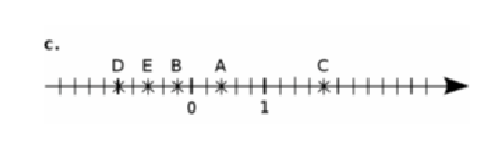
\includegraphics[scale=1]{abscisses2.eps} 

\emul

\q Donner les coordonnées des points A, D, C et E.\\

\includegraphics[scale=1]{coordonnées.eps} \\

\q A l'aide du repère ci-dessus, placer les points suivants : G(4; 4) ; H(-1; 5) ; I(-6; 0) ; J(5; 5;-1).\\




\exo{6} 

\bmul{2}
Des enfants lancent 4 fléchettes sur la cible représentée ci-contre.\\
On obtient :\\
\bi
\item 5 points pour un tir dans le rouge,
\item 2 points pour un tir dans le vert,
\item -1 point pour un tir dans le bleu,
\item -10 points si on rate la cible.
\ei

\columnbreak

\begin{center}
 
\includegraphics[scale=1]{cible.eps}
 \end{center} 
\emul

Voici les résultats des 4 compétiteurs :\\
\bmul{2}
\noindent Anaïs : rouge, vert, vert, raté\\
David : rouge, vert, bleu, raté

\columnbreak

\noindent Eva : rouge, raté, raté, rouge\\
Sacha : vert, vert, bleu, raté

\emul

\initq
\q 
\qa Écrire l'expression qui permet de calculer le score de chaque enfant, puis calculer ce score.\\

\qa Ranger ces scores par ordre croissant.\\

\q Un enfant a obtenu le score de -31. Quels sont ses 4 lancers ?\\

\vspace*{0.5cm}

\exo{2} Dans la figure ci-dessous, les quadrilatères ACBD et EFHG sont symétriques par rapport au point O.

\begin{center}
 \includegraphics[scale=1]{quadrilatere.eps}\\
 \end{center} 

\initq
\q Quel est le symétrique de point B par rapport au point O.\\

\q Quel est le symétrique du segment [AD] par rapport au point O.\\

\q Quel est le symétrique de la droite (FH) par rapport au point O.\\

\q Quel est le symétrique de la droite (FG) par rapport au point O.\\




\exo{3,5}

\initq 
\q Construire un triangle ABC rectangle en A tel que  : AB = 6cm et AC = 4cm.\\

\q Construire sur la même figure en utilisant trois couleurs différentes, les triangles symétriques du triangle ABC par rapport : 

\bmul{3}
a. au point A

\columnbreak

b. au point B
\columnbreak

c. au point C
\emul

\exo{2}\\

Après avoir reproduit ce dessin sur ta copie, complète-le en faisant le symétrique de chaque figure par rapport au point O.\\

\begin{center}
\includegraphics[scale=1]{figure.eps} 
\end{center}



\end{document}
